\documentclass[ignorenonframetext,]{beamer}
\setbeamertemplate{caption}[numbered]
\setbeamertemplate{caption label separator}{: }
\setbeamercolor{caption name}{fg=normal text.fg}
\beamertemplatenavigationsymbolsempty
\usepackage{lmodern}
\usepackage{amssymb,amsmath}
\usepackage{ifxetex,ifluatex}
\usepackage{fixltx2e} % provides \textsubscript
\ifnum 0\ifxetex 1\fi\ifluatex 1\fi=0 % if pdftex
  \usepackage[T1]{fontenc}
  \usepackage[utf8]{inputenc}
\else % if luatex or xelatex
  \ifxetex
    \usepackage{mathspec}
  \else
    \usepackage{fontspec}
  \fi
  \defaultfontfeatures{Ligatures=TeX,Scale=MatchLowercase}
\fi
\usetheme[]{AnnArbor}
% use upquote if available, for straight quotes in verbatim environments
\IfFileExists{upquote.sty}{\usepackage{upquote}}{}
% use microtype if available
\IfFileExists{microtype.sty}{%
\usepackage{microtype}
\UseMicrotypeSet[protrusion]{basicmath} % disable protrusion for tt fonts
}{}
\newif\ifbibliography
\hypersetup{
            pdftitle={Bound together or loose ends?},
            pdfauthor={Pratik R Gupte, Selin Ersoy \& Allert I Bijleveld},
            pdfborder={0 0 0},
            breaklinks=true}
\urlstyle{same}  % don't use monospace font for urls

% Prevent slide breaks in the middle of a paragraph:
\widowpenalties 1 10000
\raggedbottom

\AtBeginPart{
  \let\insertpartnumber\relax
  \let\partname\relax
  \frame{\partpage}
}
\AtBeginSection{
  \ifbibliography
  \else
    \let\insertsectionnumber\relax
    \let\sectionname\relax
    \frame{\sectionpage}
  \fi
}
\AtBeginSubsection{
  \let\insertsubsectionnumber\relax
  \let\subsectionname\relax
  \frame{\subsectionpage}
}

\setlength{\parindent}{0pt}
\setlength{\parskip}{6pt plus 2pt minus 1pt}
\setlength{\emergencystretch}{3em}  % prevent overfull lines
\providecommand{\tightlist}{%
  \setlength{\itemsep}{0pt}\setlength{\parskip}{0pt}}
\setcounter{secnumdepth}{0}

\title{Bound together or loose ends?}
\author{Pratik R Gupte, Selin Ersoy \& Allert I Bijleveld}
\date{September 26, 2018}

\begin{document}
\frame{\titlepage}

\section{Introduction}\label{introduction}

\begin{frame}{Waders in the Wadden Sea}

Waders such as red knots \emph{Calidris canutus} gather in large
non-breeding flocks in the Wadden Sea, where they forage on the
intertidal mudflats

\begin{figure}
\includegraphics[width=400px]{/home/pratik/git/knots/knots_texts/fig_mudflats} \caption{Wadden Sea mudlfats}\label{fig:unnamed-chunk-1}
\end{figure}

\end{frame}

\begin{frame}{Knots benefit from sociality}

Knots can use social information in lab settings to find
food\textsuperscript{{[}1{]}}, and may learn the location of profitable
foraging patches by observing flock-mates\textsuperscript{{[}2{]}}

 1: Bijleveld et al. 2015. \emph{Behav. Processes} 2: Bijleveld et al.
2010. \emph{Oikos}

\end{frame}

\begin{frame}{Do knots have friends?}

Knots benefit from association, but do they have friends --- persistent,
non-random associations --- within \& between tidal
intervals\textsuperscript{{[}3{]}{[}4{]}}?

 3: Myers 1983. \emph{Behav. Ecol. Sociobiol.} 4: Conklin \& Colwell
2007. \emph{J. Field. Ornith.}

\end{frame}

\section{Methods}\label{methods}

\begin{frame}{ATLAS tracking}

We set up ATLAS --- a tracking system based on the \textbf{T}ime
\textbf{o}f \textbf{A}rrival (\textbf{ToA}) of radio signals from tags

\begin{figure}
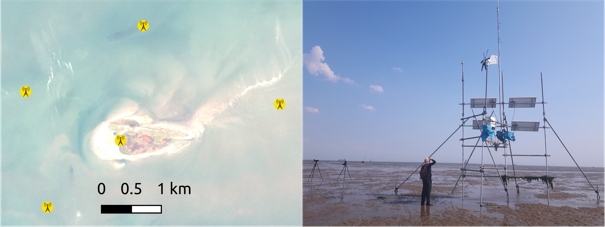
\includegraphics[width=300px]{~/git/knots/knots_texts/tracking_tower_map} \caption{Tracking tower and locations}\label{fig:unnamed-chunk-2}
\end{figure}

\end{frame}

\begin{frame}{Tidal intervals}

\begin{itemize}
\tightlist
\item
  We obtained water-level data and determined tidal intervals --- 44
  tidal intervals over 19 calendar days;
\item
  We grouped each knot's movement tracks by the tidal interval
\end{itemize}

\end{frame}

\end{document}
